\documentclass{beamer}
\usepackage[latin1]{inputenc}
\usetheme{Warsaw}
\usepackage{lipsum}

\usepackage{algorithm,algorithmic}

\setbeamercolor*{item}{fg=red}
\setlength{\leftmargini}{0pt}
\title[Regularized Logistic Regression using Gradient Descent]{Regularized Logistic Regression using Gradient Descent}
\author{Abhishek, Mirza Galib A H Baig}

\institute{Indian Institute of Technology Guwahati}
\date{November 19, 2015}
\begin{document}

\begin{frame}
\titlepage
\end{frame}

\begin{frame}{Regularized Logistic Regression: Intuition}
\begin{itemize}
	\item We want to find the  $Pr(Y=1|x)$ as a function of x i.e $\sigma$($\theta^{T}x$). 
	\item Unknown parameter ($\theta$) in the function is learned by minimizing  $J(\theta)  =-1/m\sum_{n=1}^{m}(y^{i}log(\sigma(\theta^{T},X^{i})) + (1-y^{i})log(1-\sigma(\theta^{T},X^{i})))$ \\
	which is derived by  maximum likelihood estimation.
\end{itemize}

	\begin{figure}
		
		\includegraphics*[width=0.5\textwidth]{images/decision_boundary.png}
\end{figure}					
\end{frame}

\begin{frame}{Serial Gradient Descent and Bottlenecks in parallelization}

\begin{columns}[T] % align columns
	\begin{column}{.73\textwidth}
\begin{algorithm}[H]
	\begin{algorithmic}
		\STATE data\_set $\leftarrow$ $File Read$
		\FOR{$i=1$ to $I$} 
		\FOR{$j=1$ to $\theta$}
		\STATE $sum$ $=0$, $ERROR =$ []
		\FOR{$rows$ to data\_set}
		\STATE $sum$ $+$$=$ $(hypothesis(row, \theta)- label)$ $*$ $row_{j}$  
		\ENDFOR
		\STATE $ERROR_{j}=$ $\alpha * sum / number\_of\_rows$
		\ENDFOR
		\STATE $\theta = \theta - ERROR$
		\ENDFOR
	\end{algorithmic}
	\caption{Pseudo-code for Gradient Decent}
\end{algorithm}		

	\end{column}%
	\hfill%

	\begin{column}{.27\textwidth}
	
	\begin{figure}
		\noindent
		\includegraphics*[width=1.3\textwidth]{images/gradient.png}

	\end{figure}
	Bottlenecks 
	\begin{itemize}
		\item Initial File read is sequential
		\item Wait for combining result
	\end{itemize}

	\end{column}%
	\hspace*{1cm}
\end{columns}


\end{frame}


\begin{frame}{Design of Parallel Gradient Descent}
	\begin{figure}[H]
		\centering
		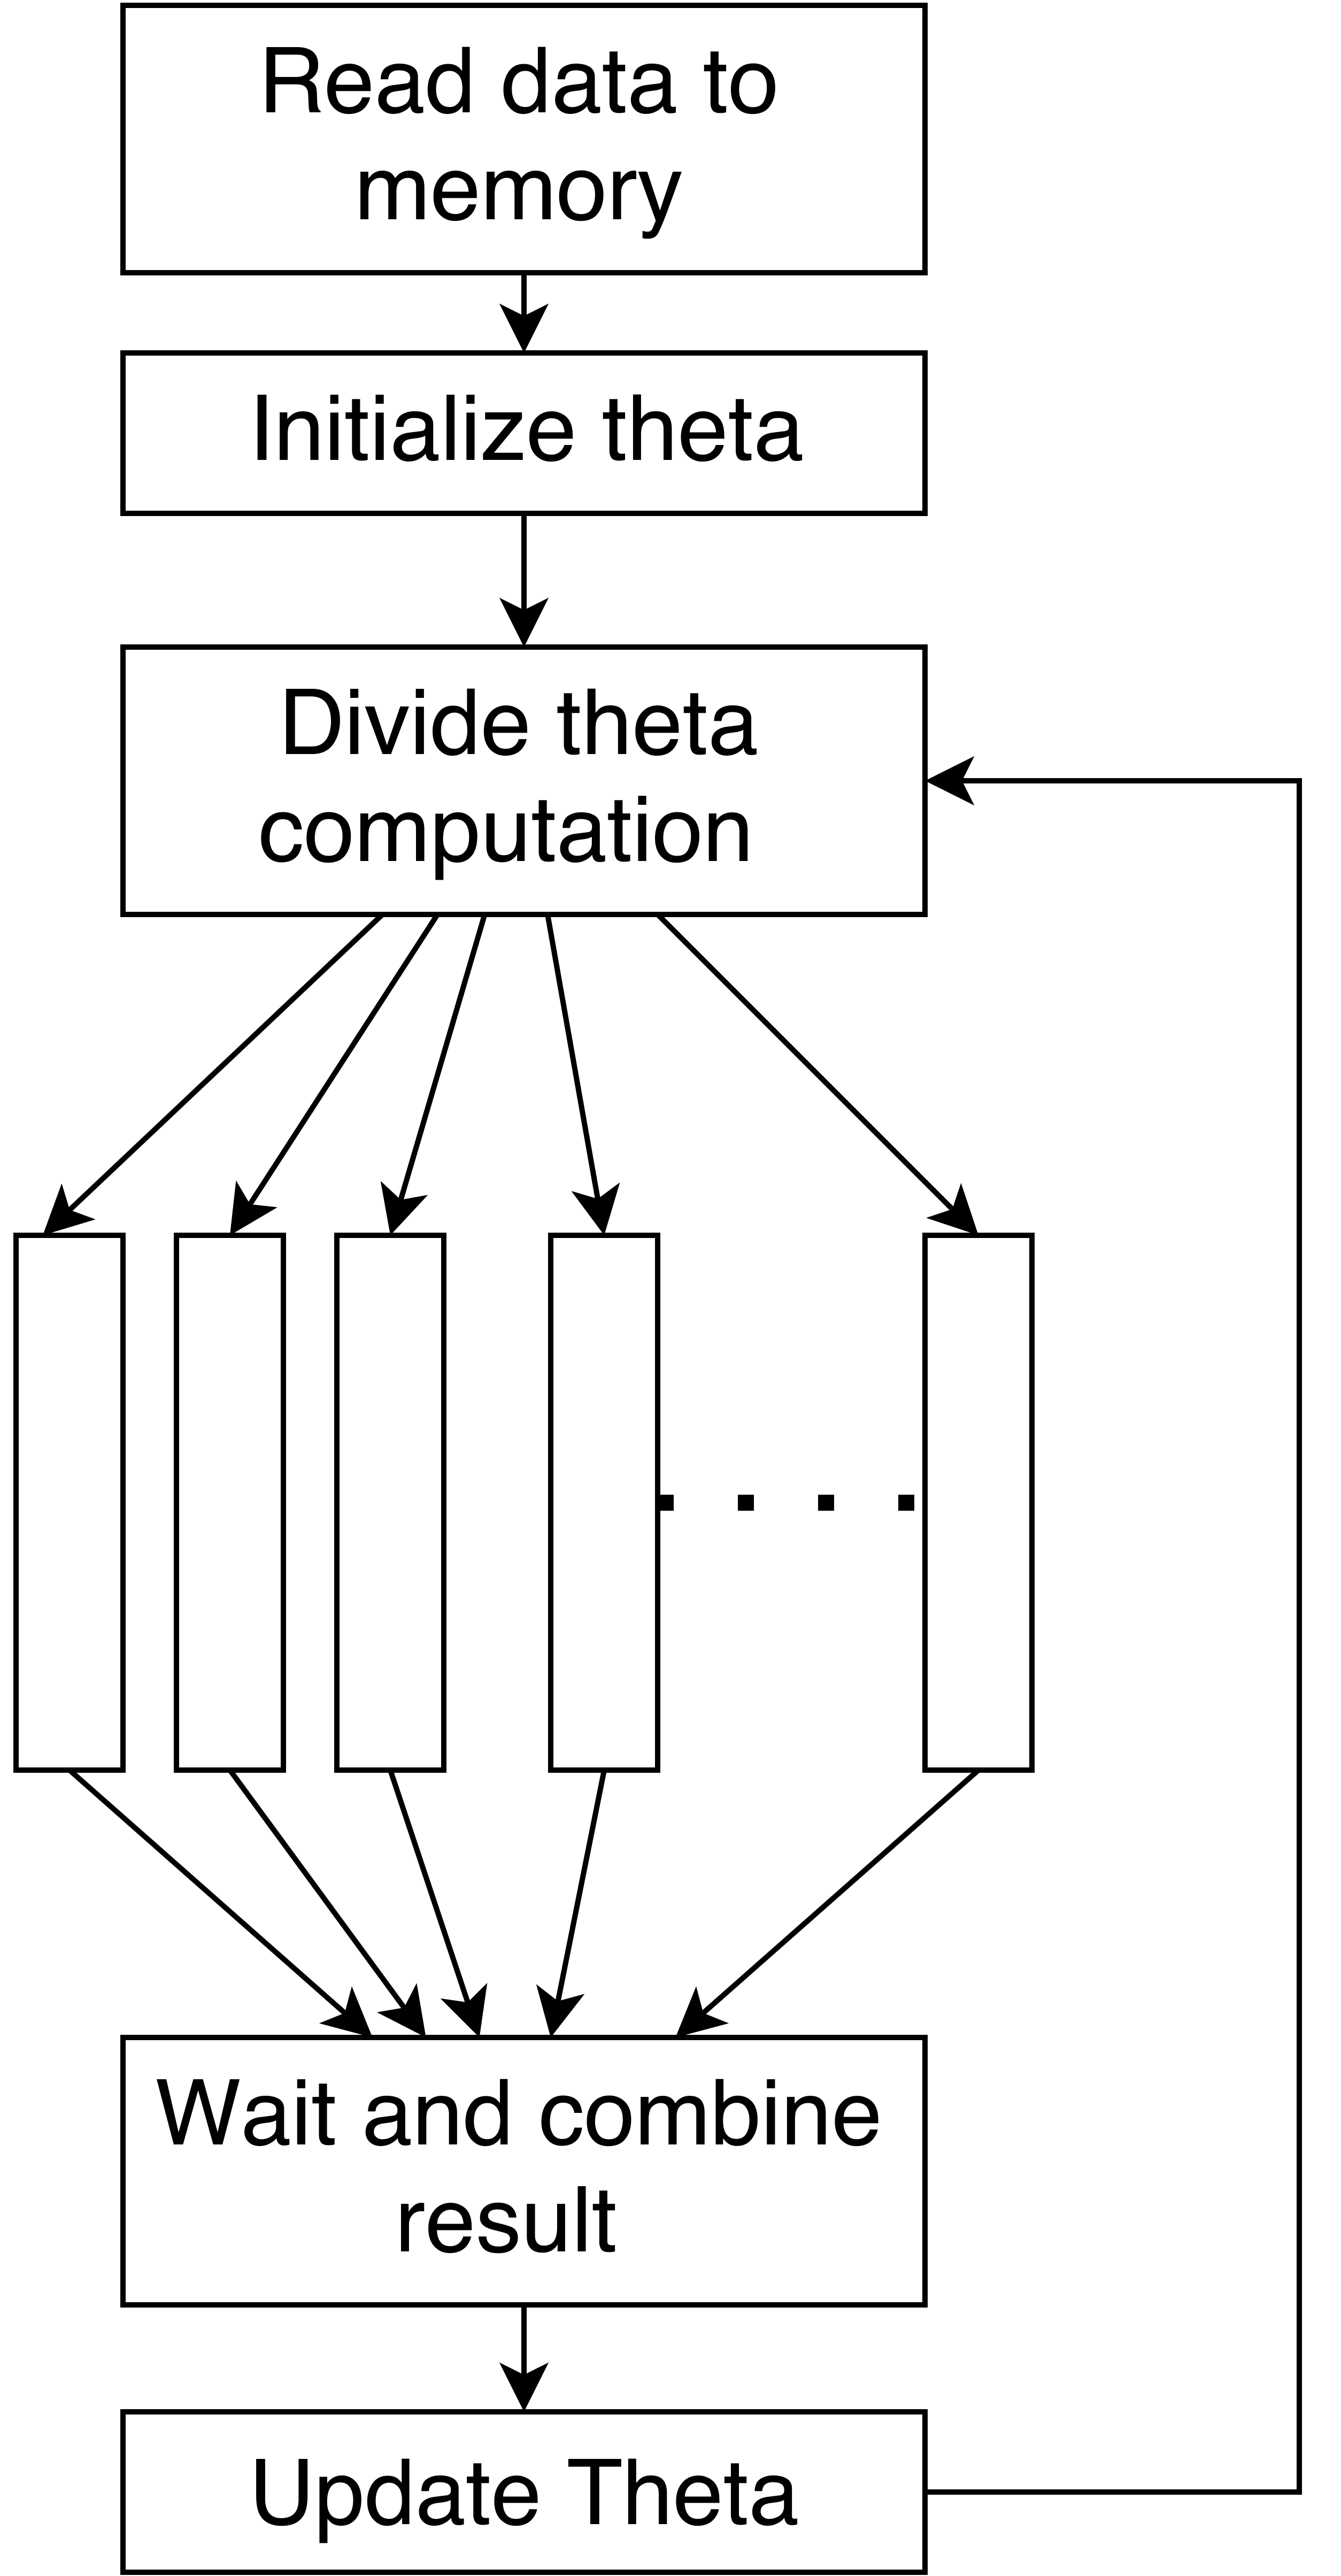
\includegraphics[width=0.35\columnwidth]{images/slide_3.png}
		\caption{Parallel Gradient Descent.}
	\end{figure}	
\end{frame}

\begin{frame}{Bottlenecks in Distributed implementation}
	\begin{itemize}
		\item Data should be divided among different nodes.
		\item Communication between different nodes.
		\item Wait till all nodes have computed before executing next iteration.
	\end{itemize}
\end{frame}

\begin{frame}{Design of Distributed Gradient Descent}
	\begin{figure}[H]
		\centering
		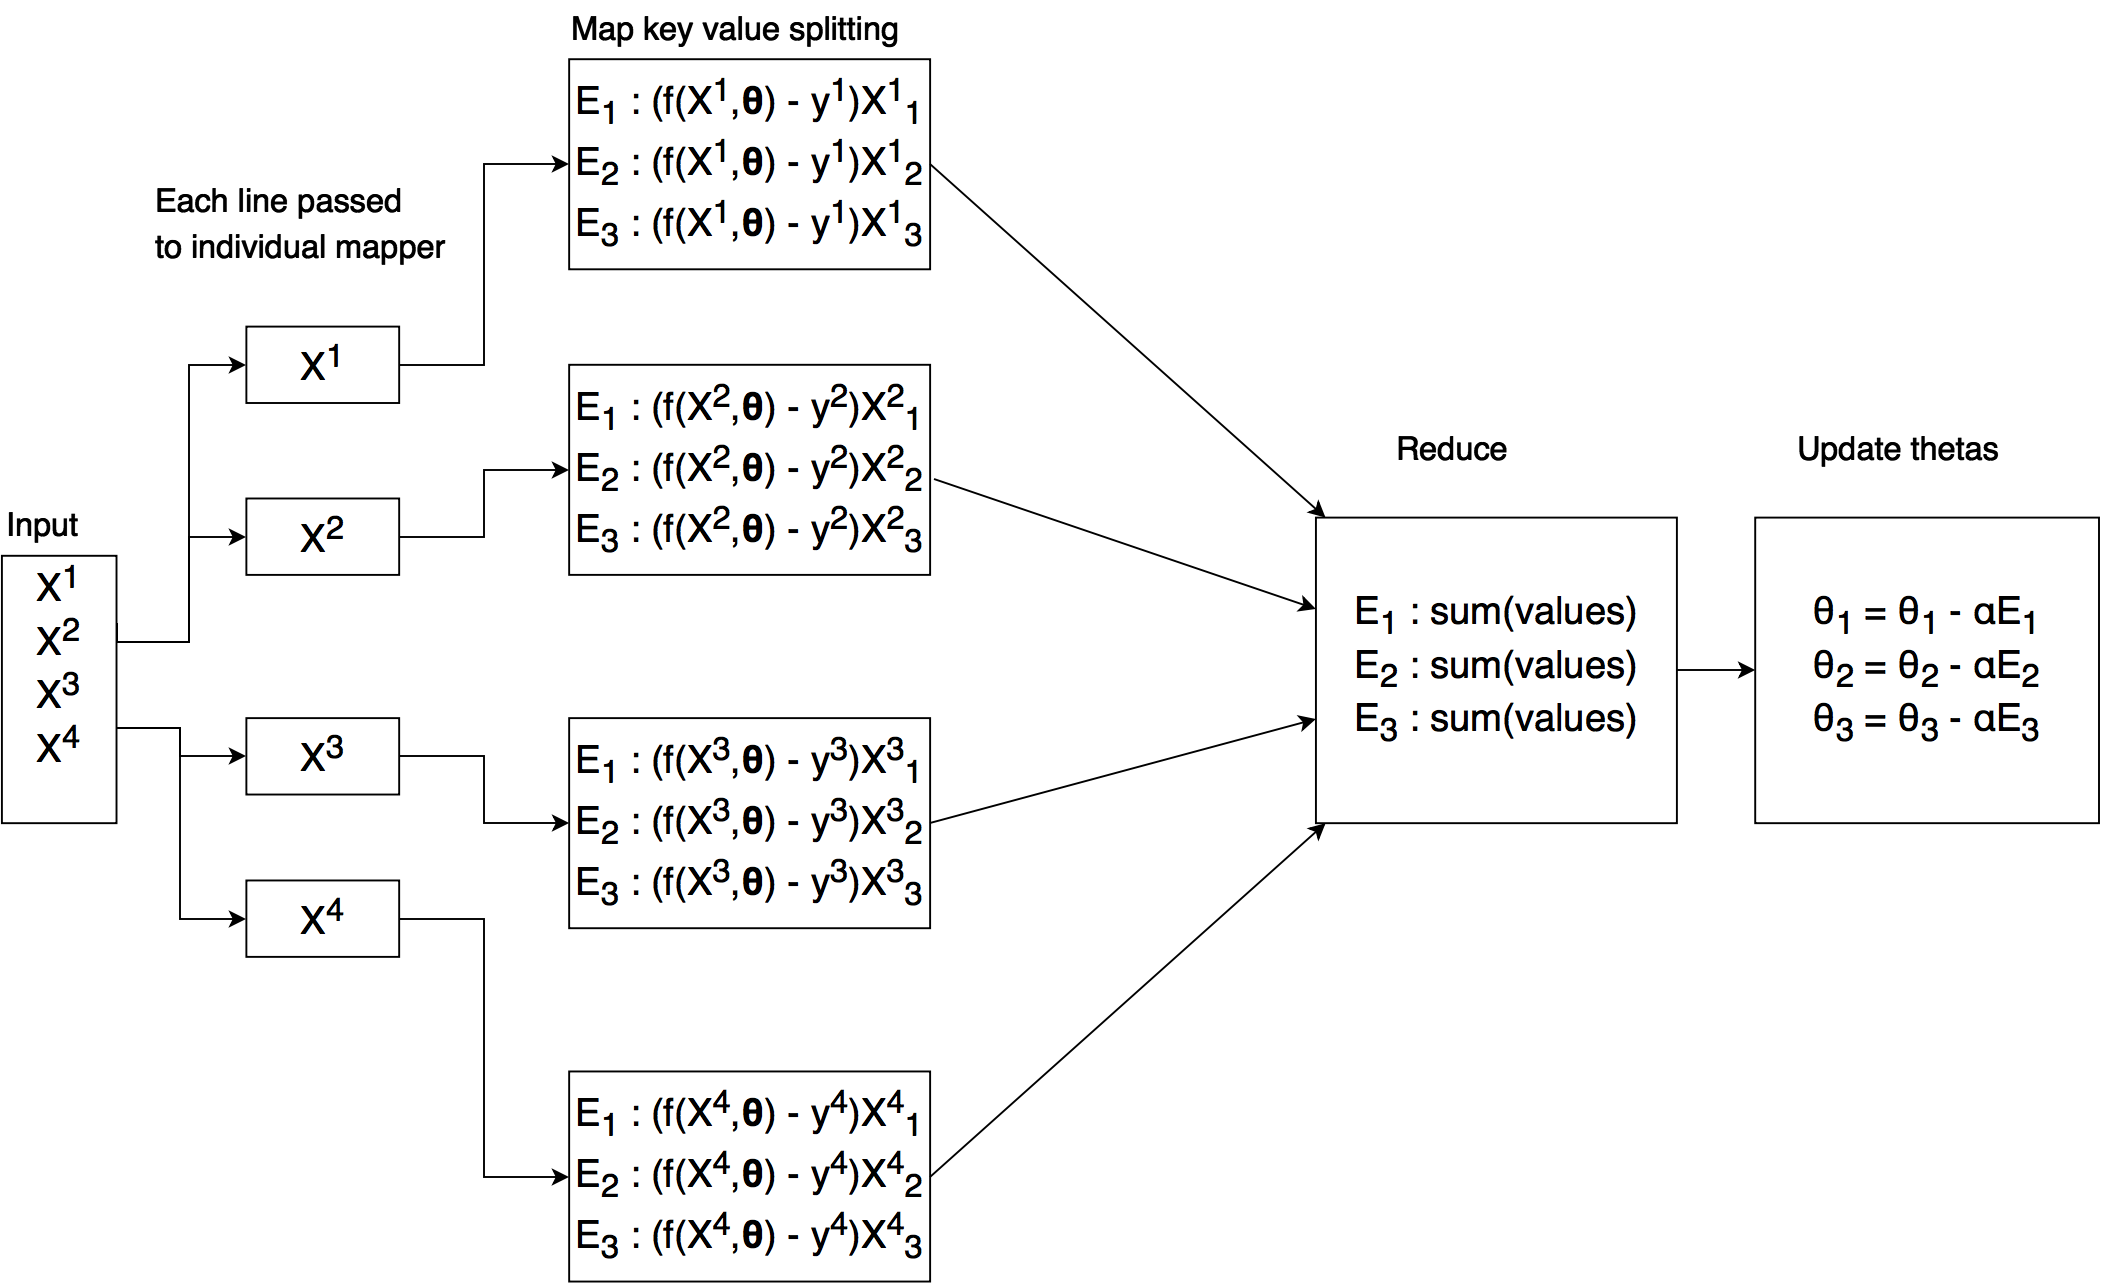
\includegraphics[width=1\columnwidth]{images/slide_5.png}
		\caption{Map Reduce Regularized Logistic Regression.}
	\end{figure}
	
\end{frame}


\end{document}